\chapter{Time series advanced metrics}
\label{sec:unchapitre}
\minitoc

\noindent Chapeau introductif
\begin{itemize}
	\item Objectif : Trouver une distance, combinaison des distances basiques qui donne une bonne classification $k$-NN sur une base de données.
	\item Pourquoi une distance combinée? Dans le cadre de données réelles, plusieurs modalités peuvent être impliquées (forme, valeur, fréquence), de manière globale ou locale.
	\item Dans le cadre des données réelles, plusieurs composantes/modalités peuvent être impliqués (forme, valeur, fréquence). = attribut (feature) en traitement du signal. Hypothèse : valeur sur une série complète, sur un intervalle ou sur une fenêtre (dans le cadre des métriques à base fréquentielle).
\end{itemize}

%-----------------------------------------------------------------------------
\section{Combined metrics for time series}
%\begin{itemize}
%	\item Certains travaux dans la littérature propose des combinaisons : linéaire, exponentielle, sigmoïde.
%	\item Limites:
%	\begin{itemize}
%		\item Implique que 2 modalités et au niveau global. Pour intégrer d'autres modalités et à d'autres échelles, il faut changer la formule et ajouter de nouveaux hyper-paramètres à optimiser $\rightarrow$ l'apprentissage de ces paramètres est plus long.
%		\item La combinaison est définie a priori
%		\item La combinaison est indépendante de la tâche d'analyse.
%		\item Pour répondre à ces problèmes, certains auteurs proposent d'apprendre une métrique en vue de la tâche d'analyse considérée (classification, régression, clustering).
%	\end{itemize}
%\end{itemize}

In most classification problems, it is not known a priori if time series of a same class exhibits same characteristics based on their amplitude,  behavior or frequential components alone. In some cases, several components (amplitude, behavior and/or frequential) may be implied. 

A first technic considers a classifier for each $p$ metric and combines the decision of the $p$ resulting classifiers. This methods is referred as post-fusion \todo{ref}, not considered in our work. Other propositions show the benefit of involving both behavior and amplitude components through a combination function. The resulting metric is then used in one classifier. This is called pre-fusion. A sigmoid combination function is proposed in~\cite{AhlameDouzal-Chouakria2011}:
\begin{equation}	
	D_{Sig}(\textbf{x}_i,\textbf{x}_j) = \frac{2d_A(\textbf{x}_i,\textbf{x}_j)}{1+\exp(\alpha cort_r(\textbf{x}_i,\textbf{x}_j))}
	\label{eq:DSig}
\end{equation}

\noindent where $\alpha$ is a parameter that defines the compromise between behavior and amplitude components. When $\alpha$ is fixed to 0, the metric only includes the value proximity component. For $\alpha \geq 6$, the metric completely includes the behavior proximity component. 

\noindent More generally, amplitude- $d_A$ and behavior- $d_{B}$ based metrics may be combined through a linear or geometric function: 
\begin{align}
D_{Lin}(\textbf{x}_i,\textbf{x}_j) &= \alpha d_{B}(\textbf{x}_i,\textbf{x}_j) + (1-\alpha) d_A(\textbf{x}_i,\textbf{x}_j)  \label{eq:DLin}   \\
D_{Geom}(\textbf{x}_i,\textbf{x}_j) &= (d_{B}(\textbf{x}_i,\textbf{x}_j))^\alpha  (d_A(\textbf{x}_i,\textbf{x}_j))^{1-\alpha} \label{eq:DGeom}
\end{align}

\noindent where $\alpha \in [0;1]$ defines the trade-off between the amplitude and the behavior components, and is thus application dependent. In general, it is learned through a grid search procedure. When $\alpha=0$, the combined metric includes only the amplitude component. For $\alpha=1$, it includes only the behavior component. 

Figs. \ref{fig:ContourLine_DLin}, \ref{fig:ContourLine_DSig} \& \todo{ref exponentiel} show the resulting metrics

However, these combinations are defined independently from the analysis task at hand. Moreover, only two variables are taking into account in these combined metrics. Finally, in the case of the model $D_{sig}$, the component $cort_r$ is a penalizing factor of $d_A$. It doesn't represent a real compromise between value and behavior components. 
% To overcome these limits, other authors propose to learn the metric $D$ for a robust $k$-NN classifier. 

\begin{figure}
	\centering
	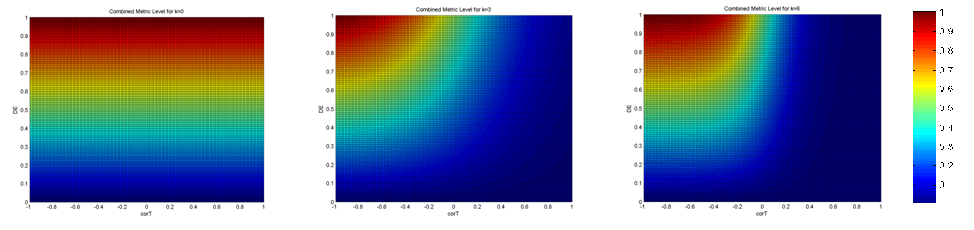
\includegraphics[width=1\linewidth]{images/ContourLine_DSig}
	\caption{}
	\label{fig:ContourLine_DSig}
\end{figure}

\begin{figure}
	\centering
	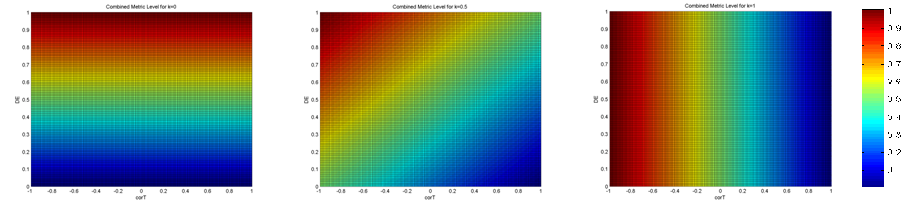
\includegraphics[width=1\linewidth]{images/ContourLine_DLin}
	\caption{}
	\label{fig:ContourLine_DLin}
\end{figure}




\newpage

%-----------------------------------------------------------------------------
\section{Metric Learning}
%\begin{itemize}
%	\item Placer le contexte : travaux réalisés dans le cadre de la classification de données statiques.
%	\item Présenter l'intuition du Metric Learning sur la base des travaux de Weinberger.
%	\item Donner la terminologie (target, imposter, push, pull)
%	\item Objectif : push des imposters et pull des targets
%	\item Formalisation du problème (optimisation)
%	\item Limites:
%	\begin{itemize}
%		\item On apprend les poids d'une distance de Mahalanobis
%		\item L'apprentissage ne prend pas en compte l'aspect multi-modal dans les données
%	\end{itemize}
%\end{itemize}

In this section, we first review a state of the art of Metric Learning. Then, we focus on the framework for Metric Learning proposed by Weinberger \& Saul for Large Margin Nearest Neighbor (LMNN) classification \cite{Weinberger2009}. We detailed the intuition, the terminology and the formalization of the optimization process.

\subsection{State of the art}
In the case of static data, many work have demonstrated that $k$-NN classification performances depends highly on the considered metric and can be improved by learning an appropriate metric \cite{Shental2002,Goldberger2004,Chopra2005}. Metric Learning can be defined as a process that aims to learn a distance from labeled examples by making closer samples that are expected to be similar, and far away those expected to be dissimilar.

\todo[inline]{A modifier, ça vient de PRL} Similar and dissimilar samples, are inherently task- and application dependent, generally given a priori and fixed during the learning process. From the surge of recent research in metric learning, one can identify mainly two categories: the linear and non linear approaches. The former is the most popular, it defines the majority of the propositions, and focuses mainly on the Mahalanobis distance learning. The latter relies on non linear Metric Learning, although more expressive, the optimization problems are more expensive to solve in general.

Contrary to flat data, Metric Learning for structured data (e.g. sequence, time series, trees, graphs) remains less numerous. While for sequence data most of the works focus on string edit
distance to learn the edit cost matrix [21, 20], Metric Learning for time series is still in its infancy. Without being exhaustive, major recent proposals rely on weighted variants of dynamic time warping to learn alignments under phase or amplitude constraints [22, 23, 24], or enlarging temporal alignments to learn discriminative matching guided by local variance/covariance [25].

In the next sections, we review the framework for Metric Learning proposed by Weinberger \& Saul for Large Margin Nearest Neighbor (LMNN) classification in the case of static data \cite{Weinberger2009}. 



\subsection{Intuition}
%\begin{itemize}
%	\item Se placer dans le contexte kNN
%\end{itemize}

The aim of Large Margin Nearest Neighbor (LMNN) framework is to learn a Mahalanobis distance for a robust $k$-NN. 

We recall that the $k$-NN decision rule will correctly classify a sample if its $k$-nearest neighbors share the same label (Section \ref{sec:kNN}). The objective of LMNN is to increase the number of samples with this property by learning a linear transformation of the input space before applying the $k$-NN classification.

Intuitively, the algorithm is based on the simple observation that the kNN decision rule will correctly classify an example if its k-nearest neighbors share the same label. The algorithm attempts to increase the number of training examples with this property by learning a linear transformation of the input space that precedes kNNclassification using Euclidean distances. The linear transformation is derived by minimizing a loss function that consists of two terms. The first term penalizes large distances between examples in the same class that are desired as k-nearest neighbors, while the second term penalizes small distances between exampleswith non-matching labels. Minimizing these terms yields a linear transformation of the input space that increases the number of training examples whose k-nearest neighbors have matching labels. The Euclidean distances in the transformed space can equivalently be viewed as Mahalanobis distances in the original space. We exploit this equivalence to cast the problem of distance metric learning as a problem in convex optimization. Our



\subsection{Problem formalization}
Let $\textbf{X}=\{\textbf{x}_i,y_i\}_{i=1}^N$ be a set of $N$ static vector samples, ${\textbf{x}_i \in \mathbb{R}^{p}}$, $p$ being the number of descriptive features and $y_i$ the class labels. Weinberger \& Saul proposed in~\cite{Weinberger2009} an approach to learn a dissimilarity metric $D$ for a large margin $k$-NN. 

It is based on two intuitions: first, each training sample $\textbf{x}_i$ should have the same label $y_i$ as its $k$ nearest neighbors; second, training samples with different labels should be widely separated. For this, they introduced the concept of \textit{target} and \textit{imposters} for each training sample $\textbf{x}_i$. \textit{Target} neighbors of $\textbf{x}_i$, noted $j \rightsquigarrow i$, are the $k$ closest $\textbf{x}_j$ of the same class $(y_j=y_i)$, while \textit{imposters} of $\textbf{x}_i$, denoted, $l \nrightarrow i$, are the $\textbf{x}_l$ of different class $(y_l \neq y_i)$ that invade the perimeter defined by the farthest targets of $\textbf{x}_i$. The \textit{target} neighborhood is defined with respect to an initial metric; the learned metric $D$ pulls the \textit{targets} and pushes the \textit{imposters} as shown in Figure \ref{fig:TargetImposterRepresentation}.

\begin{figure}[h!]
	\begin{minipage}[b]{1.0\linewidth}
		\centering
		\centerline{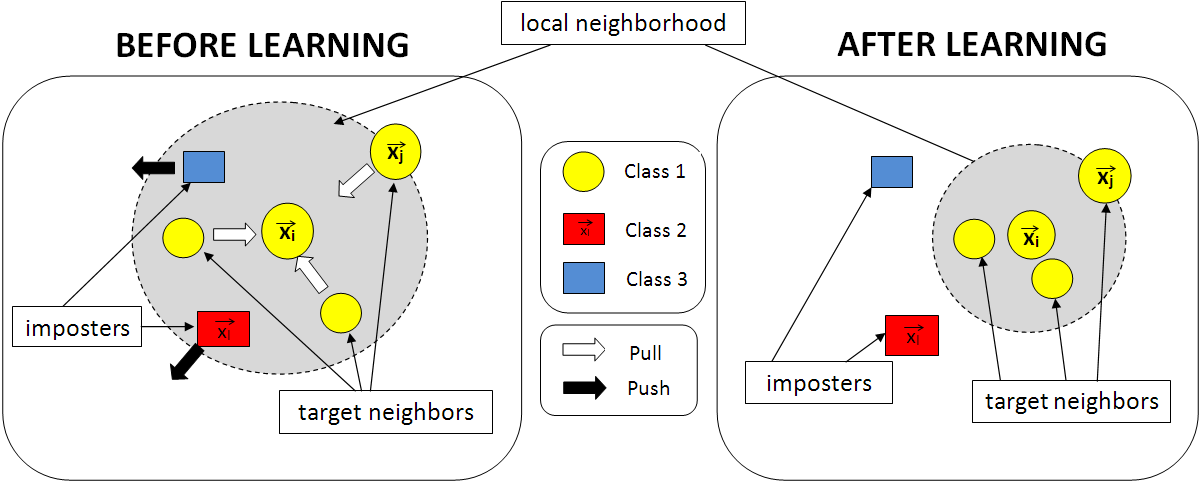
\includegraphics[width=0.8\linewidth]{./images/TargetImposterRepresentationCao}}
	\end{minipage}
	\caption{Pushed and pulled samples in the $k=3$ target neighborhood of $\textbf{x}_i$ before (left) and after (right) learning. The pushed (vs. pulled) samples are indicated by a white (vs. black) arrows (Weinberger \& Sault~\cite{Weinberger2009}).}
	\label{fig:TargetImposterRepresentation}
\end{figure}

\noindent The problem is formalized as follow:
\begin{equation}
	\begin{aligned}
	&\displaystyle 		\min_{w,\xi}\underbrace{
		\sum\limits_{i,j \rightsquigarrow i}
		D(\textbf{x}_{i},\textbf{x}_{j})
	}_{pull}
	+
	\underbrace{
		C\sum\limits_{i,j \rightsquigarrow i,l} \frac{1+y_{il}}{2}.\xi_{ijl}
	}
	_{push} \\
	&\text{s.t.  } \forall j \rightsquigarrow i, y_l\neq y_i, \\
	& D(\textbf{x}_{i},\textbf{x}_{l})-D(\textbf{x}_{i},\textbf{x}_{j}) \geq 1-\xi_{ijl} \\
	& \xi_{ijl} \geq 0 \\
	\label{eq:OptimizationProblem}
	\end{aligned}
\end{equation}
\noindent where $C$ is a trade-off between the push and pull term. Generally, the parameter $C$ can be tuned via cross validation and grid search.


There are many parallels between our method and classification by support vector machines
(SVMs)—most notably, a convex objective function based on the hinge loss, and the potential to work in nonlinear feature spaces by using the “kernel trick”. In light of these parallels, we describe our approach as large margin nearest neighbor (LMNN) classification. Our framework can be viewed as the logical counterpart to SVMs inwhich kNNclassification replaces linear classification. Our framework contrasts with classification by SVMs, however, in one intriguing respect: it
requires no modification for multiclass problems. Extensions of SVMs to multiclass problems typically involve combining the results of many binary classifiers, or they require additional machinery that is elegant but non-trivial (Crammer and Singer, 2001). In both cases the training time scales at least linearly in the number of classes. By contrast, our framework has no explicit dependence on the number of classes.

In the following, we extend this framework to learn a combined metric for a large margin $k$NN.


%Metric learning framework can be defined as learning, from the
%data and for a task, a pairwise function (i.e. a similarity, dissimilarity
%or a distance) to make closer samples that are expected
%to be similar, and far away those expected to be dissimilar.
%Similar and dissimilar samples, are inherently task- and
%application-dependent, generally given a priori and fixed during
%the learning process. From the surge of recent research in
%2
%metric learning, one can identify mainly two categories: the linear
%and non linear approaches. The former is the most popular,
%it defines the majority of the propositions, and focuses mainly
%on the Mahalanobis distance learning. The latter addresses non
%linear metric learning, although more expressive, the optimization
%problems are more expensive to solve in general.



%%% Local Variables: 
%%% mode: latex
%%% TeX-master: "../roque-phdthesis"
%%% End: 
